\pdfobjcompresslevel=0\relax
\pdfminorversion=5\relax
\documentclass[a4paper,10pt]{article}

% ---------------------------------------------------------------------
% Language, fonts and page layout
% ---------------------------------------------------------------------
\usepackage[utf8]{inputenc}
\usepackage[T5]{fontenc}
\usepackage{lmodern}
\usepackage[english]{babel}
\usepackage{microtype}

\usepackage[a4paper,left=19mm,right=19mm,top=22mm,bottom=22mm]{geometry}
\usepackage{indentfirst}

% ---------------------------------------------------------------------
% Tables, figures, colour
% ---------------------------------------------------------------------
\usepackage{float}
\usepackage{array}
\usepackage{tabularx}
\usepackage{booktabs}
\usepackage{multirow}
\usepackage{graphicx}
\usepackage{adjustbox}
\usepackage{caption}
\usepackage{amsmath}
\usepackage{xcolor}
\usepackage{tikz}
\usetikzlibrary{arrows.meta,calc}
\usepackage{enumitem}
\setlist{nosep,leftmargin=1.4em,itemsep=1pt,topsep=2pt}

\newcolumntype{L}[1]{>{\raggedright\arraybackslash}p{#1}}
\newcolumntype{Y}{>{\raggedright\arraybackslash}X}

% Section spacing (compact, but with a clear gap above each heading).
\makeatletter
\renewcommand\section{\@startsection{section}{1}{\z@}%
                                   {-11pt \@plus -2pt \@minus -1pt}%
                                   {4pt \@plus 1pt \@minus 1pt}%
                                   {\normalfont\large\bfseries}}
\renewcommand\subsection{\@startsection{subsection}{2}{\z@}%
                                     {-8pt \@plus -1pt \@minus -1pt}%
                                     {3pt \@plus 1pt \@minus 1pt}%
                                     {\normalfont\normalsize\bfseries}}
\makeatother
\setlength{\parskip}{1.5pt plus 0.5pt minus 0.5pt}
\setlength{\parindent}{12pt}
\setlength{\emergencystretch}{3em}

% ---------------------------------------------------------------------
% Bibliography and hyperlinks
% ---------------------------------------------------------------------
\usepackage[numbers,sort&compress]{natbib}
\bibliographystyle{plainnat}
\usepackage[unicode,breaklinks,plainpages=false,pdfpagelabels]{hyperref}
\hypersetup{
    colorlinks=true,
    linkcolor=blue!50!black,
    citecolor=blue!50!black,
    urlcolor=blue!50!black,
    pdftitle={LuatCheck: D2 Interim Report (CO5151, Group 8)},
    pdfauthor={CO5151 Group 8}
}

% ---------------------------------------------------------------------
% Header and footer
% ---------------------------------------------------------------------
\usepackage{fancyhdr}
\setlength{\headheight}{36pt}
\pagestyle{fancy}
\fancyhead{}
\fancyhead[L]{%
 \begin{tabular}{rl}
    \begin{picture}(25,15)(0,0)
        \put(0,-8){
\includegraphics[width=8mm]{images/hcmut.png}}
    \end{picture}
    &
    \begin{tabular}{l}
        \textbf{\ttfamily VIETNAM NATIONAL UNIVERSITY HO CHI MINH CITY}\\
        \textbf{\ttfamily HO CHI MINH CITY UNIVERSITY OF TECHNOLOGY}
    \end{tabular}
 \end{tabular}
}
\fancyhead[R]{}
\fancyfoot{}
\fancyfoot[L]{\scriptsize\ttfamily CO5151 · Advanced Agentic Artificial Intelligence · D2 Interim Report}
\fancyfoot[R]{\scriptsize\ttfamily Page \thepage}
\renewcommand{\headrulewidth}{0.3pt}
\renewcommand{\footrulewidth}{0.3pt}

\captionsetup{font=small,labelfont=bf,aboveskip=4pt,belowskip=2pt}
\setlength{\floatsep}{8pt plus 2pt minus 2pt}
\setlength{\textfloatsep}{8pt plus 2pt minus 2pt}
\setlength{\intextsep}{8pt plus 2pt minus 2pt}

% ---------------------------------------------------------------------
% Macros
% ---------------------------------------------------------------------
% Run-in paragraph heading.
\newcommand{\hdr}[1]{\par\smallskip\noindent\textbf{#1}}
% Red placeholders: every missing result, input or decision uses one of these two macros
% (the generated tables use the identical red bold [PENDING] marker).
\newcommand{\pending}[1]{\textcolor{red}{\textbf{[PENDING: #1]}}}
\newcommand{\tbd}{\textcolor{red}{\textbf{[PENDING]}}}
% Code identifiers and paths (not hyperlinked) and shell commands (spaces preserved).
\newcommand{\code}[1]{\nolinkurl{#1}}
\newcommand{\cmd}[1]{\texttt{\detokenize{#1}}}
% Table style shared by all hand-written tables.
\newcommand{\tabstyle}{\centering\footnotesize\renewcommand{\arraystretch}{1.05}\setlength{\tabcolsep}{3.5pt}}

% The generated result tables use \resizebox{\textwidth}{!}{...}, which also scales narrow tables up.
% Cap the width instead: a narrow table keeps its natural size, a wide one shrinks to the text width.
\renewcommand{\resizebox}[3]{\adjustbox{max width=#1}{#3}}

% \inputhere: input a generated table file but place its floats where they appear (the renderer emits [t]).
\makeatletter
\newcommand{\inputhere}[1]{\begingroup\renewcommand\table[1][]{\@float{table}[!htb]}\input{#1}\endgroup}
\makeatother

\begin{document}
\hypersetup{pageanchor=false}
\begin{titlepage}\begin{center}
\textbf{VIETNAM NATIONAL UNIVERSITY HO CHI MINH CITY}\\
\textbf{HO CHI MINH CITY UNIVERSITY OF TECHNOLOGY}\\
\textbf{FACULTY OF COMPUTER SCIENCE AND ENGINEERING}\\[15pt]

\includegraphics[width=2.7cm]{images/hcmut.png}\\[15pt]
{\Large CO5151 -- Advanced Agentic Artificial Intelligence}\\[12pt]
{\Huge\bfseries D2 Interim Report}\\[12pt]
{\Large LuatCheck: A Local, Source-Grounded Assistant\\ over Vietnamese Regulations}\\[12pt]
Application Track -- Group 8\\[15pt]
\pending{Draft of 23 October 2026. All result tables stay empty until the main runs, the judge audit and the team's inputs exist.}\\[15pt]
\begin{tabular}{ll}
Instructor & TS. Lê Xuân Bách\\
Members & Lê Trí Quyền (2470740)\\
& Võ Phạm Tuấn Dũng (2570015)\\
& Nguyễn Hoàng Phong (2570477)
\end{tabular}\\[18pt]
\textbf{Repository:} \url{https://github.com/tuandung222/LuatCheck-D2}\\[8pt]
\textbf{Reported revision:} \pending{Insert the full final commit hash after freezing the source.}\\[8pt]
\textbf{Access:} \pending{Confirm the instructor can read the repository.}\\[8pt]
\textbf{Status:} At risk (provisional). The benchmark design is frozen and the pipeline is in place; main-run results, the human audit of the judge and the demo rehearsal are outstanding.
\vfill HO CHI MINH CITY, OCTOBER 2026
\end{center}\end{titlepage}
\hypersetup{pageanchor=true}\setcounter{page}{1}

\begin{center}
\fbox{\parbox{\dimexpr\textwidth-2\fboxsep-2\fboxrule\relax}{\small
\textbf{Summary.} LuatCheck is a local agent that answers only from a document collection, cites the sections it used, checks those citations in code, and refuses or asks a clarifying question when the sources do not answer. One bounded agent loop drives a 2B ternary controller that fits a 16\,GiB Mac.\par\smallskip
\textbf{Implemented:} the loop, a read-only tool layer with gated writes, lexical citation checking (L1) with bounded repair, an optional cross-encoder reranker, two ingested corpora (academic regulations of the Ho Chi Minh City University of Technology, HCMUT, and Vietnamese labour-law texts) and a one-command, hash-locked benchmark pipeline (Sections~\ref{sec:arch}--\ref{sec:memory}).\par\smallskip
\textbf{Evaluation design, frozen but not yet run:} two 50-task benchmarks $\times$ three variants (OFF: no verification; L1: lexical verification with repair; L1+rerank: L1 plus reranker) $\times$ three seeds, plus two diagnostic baselines (closed-book and oracle, one seed, not system variants), scored by a large language model (LLM) judge whose reliability is to be checked against human labels (Section~\ref{sec:eval}).\par\smallskip
\textbf{Pending, in red throughout:} the results of the planned 1,090 trials (900 system plus 190 baseline), the judge audit, member contribution evidence, the commit hash and the demo rehearsal. Self-assessment: \textbf{at risk} (Section~\ref{sec:plan}).}}
\end{center}

\section{Changes from the Proposal}\label{sec:changes}
\hdr{Scope and users.} The proposal (D1, Application Track) targeted employees and small-business HR staff asking labour-law questions. For D2 we added a second, non-legal corpus: the academic-affairs regulations of HCMUT, used by students and advisors. It tests whether the code is domain-agnostic, since domain wording, tool names and ID rules live in \code{config/domains/} as data. We claim only what is evaluated: ten HCMUT regulations and ten labour-law documents (the 2019 Labour Code and nine laws, decrees and circulars of 2020--2025), snapshotted on 22 October 2026 with later amendments unchecked. LuatCheck is not legal advice and has not been tried by real users.

\hdr{Scenarios.} (1) A student looks up a rule (e.g.\ make-up class registration) and opens the cited section. (2) An employee or HR officer asks a labour-law question and checks the cited article. (3) A careless or malicious user pastes a document with injected instructions, or asks how to evade a rule; the system must hold its tool boundary and clarify or refuse. These are intended uses, not user-study results.

\hdr{Commitments and their state.} Table~\ref{tab:commit} compares the D1 commitments due at the D2 checkpoint (week 7) with their current state.
\begin{table}[!htb]\tabstyle
\begin{tabularx}{\textwidth}{@{}L{3.5cm}L{1.7cm}Y@{}}
\toprule Proposal commitment (D1) & State & Delta and reason\\\midrule
Budgeted loop, schema output, L1 citation check & Done & Runs end to end (Section~\ref{sec:arch}); budgets and failure semantics unchanged.\\
Qwen3-4B/8B controllers; 32B comparator & Dropped & The controller is Ternary Bonsai 2 2B (GGUF). It fits a 16\,GiB Mac and one GPU slot, so the same weights serve the benchmark and the demo. A 20-trial diagnostic on the earlier task set ran about $2\times$ faster than the MLX build (\code{gguf2b-bonsai-diag-v1}).\\
BM25 + Qdrant dense retrieval; 200 held-out VLQA pairs & Dropped & Replaced by BM25 + TF-IDF fused by reciprocal rank fusion (RRF). The persisted vector index exists but is not used in D2 runs. The VLQA record mapping could not be established, so retrieval is measured as source-ID metrics on the new benchmarks.\\
$\ge$10 end-to-end tasks; 3 configurations $\times$ 3 seeds & In progress & Two frozen 50-task benchmarks, variants OFF / L1 / L1+rerank, seeds 42, 123 and 2026 (900 planned system trials per machine run), plus 190 planned diagnostic-baseline trials. Collection pending: \tbd.\\
Reranker (optional in D1) & In progress & Implemented and wired as variant L1+rerank; parity of its two runtimes pending (Section~\ref{sec:memory}).\\
L2 entailment with natural language inference (NLI), optional & In progress & Implemented as optional components; excluded from all D2 runs.\\
Guarded \code{send_summary}, UI, audit log & Done & Changed: the model can only propose; a trusted UI approves an exact payload; reversible local outbox, no sender.\\
Verifier audit (30 pairs) & Not started & Changed: replaced by a human audit of the LLM judge (about 30 items per benchmark), scheduled for Sat 24 Oct: \tbd.\\
Threat model v1 & Done & Updated in Section~\ref{sec:threat}.\\
First injection results & Not started & Not required in D2; planned for W47.\\
HR walkthrough (W5) & Not started & Reported by the group on 22 October. \pending{New date and owner.}\\
\bottomrule\end{tabularx}
\caption{D1 commitments due at the D2 checkpoint and their state (done, in progress, not started, dropped).}\label{tab:commit}
\end{table}

\hdr{Feedback and earlier pilot.} The group received no feedback on the D1 pitch (22 October), so no change is attributed to feedback. An earlier pilot (Qwen2.5-3B on Ollama, ten-task \code{bll2019_v1}) is superseded; none of its numbers appears here.

\hdr{Models and framework.} Table~\ref{tab:models} lists the components behind the reported numbers. We use no agent framework. The loop, action validation, tool registry, verifier, ledger, memory and harness are our own code (AI-assisted coding is disclosed in Section~\ref{sec:contrib}), built on \code{rank-bm25}, scikit-learn, \code{pypdf}, the Model Context Protocol (MCP) SDK, FastAPI/React and Streamlit.
\begin{table}[!htb]\tabstyle
\begin{tabularx}{\textwidth}{@{}L{2.5cm}L{5.7cm}Y@{}}
\toprule Component & Choice & Runtime and role\\\midrule
Controller & Ternary Bonsai 2 2B, GGUF, PQ2\_0 quantisation (\code{prism-ml/Ternary-Bonsai-2-2B-gguf}; file SHA-256 \code{d5f01a4e}\ldots) & PrismML fork of \code{llama.cpp}, commit \code{73bfe6c}; Metal on the Mac, CUDA on server 82 (\pending{result of the PQ2\_0-on-CUDA gate}). Used for every reported number and for the live demo.\\
Reranker & \code{AITeamVN/Vietnamese_Reranker}, cross-encoder, revision \code{f5369762} (weights SHA-256 \code{1cecccab}\ldots) & Variant L1+rerank only: torch fp16 on server 82, a GGUF conversion on the Mac.\\
First-stage retrieval & BM25 + TF-IDF fused by RRF; no neural embeddings & In memory; all variants.\\
Judge & DeepSeek V4.1 Flash & Through an API gateway; offline evaluation only.\\
\bottomrule\end{tabularx}
\caption{Models and software behind the reported numbers. Server 82 is the shared GPU server (one H100 used).}\label{tab:models}
\end{table}
Controller sampling is fixed: temperature 0.7, top-p 0.8, top-k 20, presence penalty 1.5, decoding constrained to the action JSON schema, thinking off, at most 1,024 output tokens. The live demo runs the same model file, \code{llama.cpp} commit, sampler, prompts, budgets and corpora, one query at a time through the web UI. It illustrates the tables; it is not evidence for them.

\section{Implemented Architecture (R1)}\label{sec:arch}
LuatCheck is a single agent running a ReAct-style loop~\citep{yao2023react} over retrieval-augmented generation~\citep{lewis2020rag} (Figure~\ref{fig:arch}). At each step the controller emits one JSON action: \code{search}, \code{read}, \code{answer}, \code{clarify} or \code{refuse}. The Python tool registry executes searches and reads and returns the result as an observation. An \code{answer} passes through the verifier; if the check fails, the verifier's feedback goes back to the controller for at most two repairs, which is external feedback rather than self-critique~\citep{huang2024selfcorrect}. Input guardrails refuse unsafe input before any model call. The loop is bounded to 8 steps, 5 tool calls, 2 repairs and 180\,s per task (60\,s per model request). A backend or model-format failure ends the run as \code{error}; it is never turned into an answer or a refusal.

There is one controller and no multi-agent coordination, which keeps permissions and budgets easy to inspect. The MCP server exposes the same tools but the loop does not use it. The three variants test whether verification and reranking help (Section~\ref{sec:eval}).
\begin{figure}[!t]\centering
% Figure 1 (architecture and control flow). Drawn at true size, 17.0 cm wide, no scaling.
% Encoding (Okabe-Ito blue/orange; every class also differs in border style or tag text, so it reads in greyscale):
%   blue fill   = part of the chosen system, always on
%   orange fill = part of the chosen system with an on/off switch (ablated in Section 5)
%   dashed      = implemented, not part of any D2 measurement
%   grey fill   = terminal state of a run
\begin{tikzpicture}[x=1cm,y=1cm,font=\scriptsize,line cap=round,
  box/.style={draw=blue!55!black,fill=blue!8,rounded corners=2pt,align=center,inner sep=3pt,minimum height=1.0cm,line width=0.6pt},
  var/.style={box,draw=orange!70!black,fill=orange!22},
  off/.style={box,dashed,draw=black!60,fill=white,text=black!70},
  term/.style={box,draw=black!70,fill=black!10},
  frame/.style={draw=black!45,fill=black!3,rounded corners=4pt,line width=0.6pt},
  flow/.style={-{Stealth[length=5pt,width=4.5pt]},line width=0.8pt},
  alt/.style={flow,dashed},
  logl/.style={-{Stealth[length=4pt,width=3.5pt]},line width=0.6pt,dotted,black!65},
  lab/.style={font=\scriptsize,inner sep=1.2pt,fill=white,fill opacity=0.92,text opacity=1}]

% loop frame and its budget label
\node[frame,minimum width=13.9cm,minimum height=6.2cm,anchor=north west] (fr) at (3.1,9.3) {};
\node[anchor=north west,align=left,font=\scriptsize\bfseries] at (3.3,9.2) {Bounded agent loop\\[-1pt]{\normalfont $\le$\,8 steps, 5 tool calls,}\\[-1pt]{\normalfont 2 repairs, 180\,s per task}};

% input column
\node[box,text width=2.0cm] (q) at (1.1,8.45) {Question or pasted document};
\node[box,text width=2.0cm] (g) at (1.1,6.5) {\textbf{Input guardrails}\\pattern checks, sanitising, untrusted tags};

% loop body
\node[box,text width=3.0cm] (c) at (5.4,6.5) {\textbf{Controller}\\Bonsai 4B (2B option), one JSON action per step};
\node[box,text width=2.0cm] (t) at (10.0,6.5) {\textbf{Tool registry}\\search, read\\read-only};
\node[box,text width=3.2cm] (r) at (15.1,8.1) {\textbf{First-stage retrieval}\\BM25 + TF-IDF, RRF\\top-20 candidates};
\node[var,text width=3.2cm] (rr) at (15.1,5.5) {\textbf{Reranker} (switch)\\cross-encoder\\top-20 $\to$ top-5};
\node[var,text width=3.0cm] (v) at (5.4,4.1) {\textbf{L1 verifier + repair} (switch)\\ids, quotes,\\overlap, quantities};
\node[off,text width=3.2cm] (l2) at (15.1,4.1) {L2 / NLI step, dense retrieval\\implemented, not evaluated};

% terminal states and side components (bottom row)
\node[term,text width=2.0cm] (ref) at (1.1,1.7) {\textbf{Refused} or \textbf{clarified}};
\node[term,text width=3.0cm] (ans) at (5.4,1.7) {\textbf{Answer} with verified citations};
\node[off,text width=2.3cm] (mem) at (9.1,1.7) {Answer memory\\(off in D2)};
\node[term,text width=2.6cm] (err) at (12.1,1.7) {\textbf{Error}: backend or budget failure, never an answer};
\node[off,text width=2.5cm] (out) at (15.7,1.7) {Trusted UI outbox\\(host approves payload)};
\node[box,fill=black!3,draw=black!60,minimum width=16.9cm,minimum height=0.7cm,anchor=south west] (led) at (0,-0.35) {\textbf{Case ledger and audit log}: queries, tool calls, ids, repairs, tokens, times};

% control flow inside the loop
\draw[flow] (q) -- (g);
\draw[flow] (g) -- (c);
\draw[flow] ([yshift=0.27cm]c.east) -- node[lab,above=1pt]{tool call} ([yshift=0.27cm]t.west);
\draw[flow] ([yshift=-0.27cm]t.west) -- node[lab,below=1pt]{observation} ([yshift=-0.27cm]c.east);
\draw[flow] ([xshift=-0.7cm]c.south) -- node[lab,left=1pt]{answer} ([xshift=-0.7cm]v.north);
\draw[flow] ([xshift=0.7cm]v.north) -- node[lab,right=1pt]{repair} ([xshift=0.7cm]c.south);
% search path: query goes out above, results come back below (nested, no crossings)
\draw[flow] ([xshift=-0.4cm]t.north) |- node[lab,pos=0.8]{query} ([yshift=0.27cm]r.west);
\draw[alt] ([yshift=-0.27cm]r.west) -| node[lab,pos=0.2]{top-5 (reranker off)} ([xshift=0.4cm]t.north);
\draw[flow] (r) -- node[lab]{top-20} (rr);
\draw[flow] (rr.west) -| node[lab,pos=0.2]{top-5 reranked} (t.south);
\draw[alt] (v.east) -- node[lab]{optional} (l2.west);

% exits
\draw[flow] (g.south) -- node[lab,pos=0.4]{unsafe} (ref.north);
\draw[flow] ([yshift=-0.27cm]c.west) -- ++(-1.1,0) coordinate (cl) |- ([yshift=0.25cm]ref.east);
\node[lab,rotate=90] at (cl |- 0,3.9) {clarify, refuse};
\draw[flow] ([yshift=-0.27cm]v.west) -- ++(-0.5,0) coordinate (rs) |- ([yshift=-0.25cm]ref.east);
\node[lab,rotate=90] at (rs |- 0,2.55) {repairs spent};
\draw[flow] (v.south) -- node[lab]{pass} (ans.north);
\draw[alt] (ans.east) -- (mem.west);
\draw[flow] (fr.south -| err) -- node[lab]{any failure} (err.north);
\draw[logl] (13.95,3.1) -- (13.95,0.35);
\end{tikzpicture}

\caption{Implemented architecture and control flow. Blue boxes run in every D2 variant; orange boxes run only in the variants they name (OFF skips the verifier; without the reranker, retrieval returns the top five directly); dashed boxes are implemented but outside every D2 run; grey boxes are the terminal states of a run. The dotted arrow marks that every step is written to the ledger.}\label{fig:arch}
\end{figure}

\hdr{What runs end to end.} Every D2 run uses input guardrails, the controller loop, \code{search} and \code{read_document}, first-stage retrieval, the ledger and the audit log. The L1 verifier with repair runs in L1 and L1+rerank, and the reranker only in L1+rerank. Four components are implemented but outside all D2 runs: the L2/NLI step, the persisted hybrid index with dense retrieval, answer memory and the trusted-UI outbox. An external sender and code execution do not exist.

\hdr{Real task trace.} A trial from the main run will be rendered from its ledger (\code{trials.jsonl}) as Table~\ref{tab:trace}. \pending{Select trial id and run id; fill the table from the recorded steps only.}
\begin{table}[!htb]\tabstyle
\begin{tabular}{@{}llllrr@{}}
\toprule Step & Action & Tool call / result ids & Verifier verdict & Tokens in/out & Time (s)\\\midrule
1 & \tbd & \tbd & \tbd & \tbd & \tbd\\
2 & \tbd & \tbd & \tbd & \tbd & \tbd\\
\ldots & \tbd & \tbd & \tbd & \tbd & \tbd\\
Total & & & & \tbd & \tbd\\
\bottomrule\end{tabular}
\caption{Trace of one completed main-run trial (task, variant, seed, run id: \tbd). Placeholder rows: nothing here is a recorded step.}\label{tab:trace}
\end{table}

\section{Tools and Permissions (R2)}\label{sec:tools}
Table~\ref{tab:tools} lists every tool and model-facing interface with its state and permission level. The controller's action space (\code{ActionType}) contains no write action, so it has no direct write path.
A stdio MCP check confirmed discovery, search, lookup, blocked unverified writes and proposal-only summaries (\code{docs/reviews/native-integrity-revision-2026-10-22}). It tests the tool contract, not a model task. The demo serves one user in one process; multi-user isolation is not certified. \pending{Attach application demo evidence from the rehearsal.}
\begin{table}[!htb]\tabstyle
% PROVENANCE: n/a descriptive tool inventory, no measured values
\begin{tabularx}{\textwidth}{@{}L{3.0cm}L{2.1cm}L{2.3cm}Y@{}}
\toprule Interface & State & Permission level & Enforced boundary\\\midrule
\code{search}, \code{read_document} (labour profile: \code{search_law}, \code{get_article}) & Implemented & Read-only & Return local corpus text only.\\
Reranker (inside \code{search}) & Implemented & Read-only (model component) & Scores candidates; a failure is an execution error (\code{ModelComponentError}), never a first-stage fallback.\\
Answer-memory write & Implemented; off in D2 & Reversible write & SQLite write only after the verification gate.\\
MCP \code{save_case} & Implemented; blocked & Reversible write & A model caller cannot self-attest verification; the call returns blocked.\\
\code{send_summary} & Proposal only & Irreversible write & The model-facing tool can only create a proposal; it cannot approve or execute.\\
Trusted-UI outbox (\code{dispatch_external_action}) & Implemented & Irreversible write (local queue only) & Needs host approval and a token bound to the payload hash; a caller flag is insufficient; a queue receipt is not a delivery.\\
External sender; code execution & Not implemented & Irreversible write; code execution & No e-mail or webhook transport and no code-running tool exists.\\
\bottomrule\end{tabularx}
\caption{Tool inventory (\code{src/tools/permissions.py}, \code{domain_tools.py}). Permission levels are those classified in code, and every non-read-only interface is blocked or gated there, not just in the prompt.}\label{tab:tools}
\end{table}

\section{Memory and Knowledge Sources (R3)}\label{sec:memory}
\hdr{Short-term context.} Each run keeps one message list: the domain system prompt, the question (and any pasted document) wrapped as untrusted input, then alternating action and tagged observation turns. Observations are compacted. \code{search} returns at most the two clauses that best match the query, plus a truncation flag; a repeated query or re-read returns a short notice; budget notices tell the model to answer or refuse. The benchmark uses an 8,192-token context, and the largest controller input in the smoke runs was 3,944 tokens. The ledger records queries, retrieved text and ids, budgets and per-call telemetry.

\hdr{Episodic memory (implemented, not exercised in D2).} Verified answers can be stored in SQLite after the verification gate. Reuse requires a matching index version, native-origin metadata and a question similarity of at least 0.85 (TF-IDF cosine and Jaccard), and the reused answer is re-verified. Memory is off in every D2 run, so trials stay independent. Reuse is also off in the demo, because matching sees only the question and not the facts that decide a case. The filter for personally identifiable information (PII) covers a fixed set of patterns.

\hdr{Knowledge sources.} \code{src/ingestion} built both corpora from public PDFs: \code{pypdf} text extraction, Unicode normalisation and segmentation at section headings. Each record carries its source URL, file SHA-256 and page numbers (manifests in \code{docs/materials/*-sources}), and IDs have the form \code{<DOC>\_<section>}. Table~\ref{tab:corpora} gives size and known limits.
\begin{table}[!htb]\tabstyle
% PROVENANCE: n/a corpus sizes counted from data/corpus, not a benchmark result
\begin{tabularx}{\textwidth}{@{}L{3.3cm}rrY@{}}
\toprule Corpus & Documents & Records & Known limits\\\midrule
\code{hcmut_academic_v1} & 10 & 143 & Several documents are amendment-only; the image-only base regulations are absent; one record has about 19,600 characters; printed decision numbers come from a web listing.\\
\code{labour_vi_v1} & 10 & 458 & Decree 145/2020 (over 40 pages) and unnumbered annexes are absent; texts as promulgated, later amendments unchecked.\\
\bottomrule\end{tabularx}
\caption{Corpora used in D2 (\code{data/corpus/}, snapshot of 22 October 2026). Neither has been certified by a domain expert: \pending{university or legal reviewer, if any}.}\label{tab:corpora}
\end{table}

\hdr{Retrieval and reranking.} Search runs in memory: BM25 over title and content and TF-IDF over word 1--3-grams, fused by RRF ($k=60$). Variants OFF and L1 return the top five first-stage results. L1+rerank takes the top 20 candidates, rescores them with the cross-encoder and returns the best five. Long records would lose late evidence if truncated, so a record longer than one window is split into overlapping windows (about 1,500 characters, 200 overlap). Each (query, window) pair is scored and the record keeps the maximum (MaxP).

The reranker's input policy and weights are identical on both machines, but the runtimes differ: torch fp16 on CUDA on server 82, and a GGUF conversion on the \code{llama.cpp} server on the Mac (quantisation: \pending{confirm after the parity check}). Scores are therefore not bit-identical: \pending{rank and score parity between the two runtimes, from the parity probe}. Accuracy comes from the GPU run and latency from the Mac run; the two L1+rerank rows are not pooled. The persisted hybrid index and dense retrieval (\code{src/indexing}) are outside D2.

\section{Evaluation Set and Initial Results (R5)}\label{sec:eval}
\hdr{Benchmarks and provenance.} \code{hcmut_v1} and \code{labour_vi_v1} each hold 50 Vietnamese tasks: 40 single-record, 5 two-record and 5 out-of-scope tasks that expect a refusal. Each task has gold record IDs, a short reference answer and verbatim evidence quotes, and both files are frozen with hashes (\code{benchmark.lock.json}). \textbf{No human wrote or reviewed any task.} Claude Haiku drafted them; two independent Claude Sonnet verifiers checked every task against the cited records; a Sonnet adjudicator fixed or replaced flagged items; mechanical checks confirmed that quotes are verbatim and IDs exist; and Gemma-4-31B answers given the gold context served as a sanity pointer (LLM estimates, not labels). The items are AI-written questions over real documents, not real user questions; real use (long, vague, pasted contracts) will differ. \pending{Member spot-check against the source PDFs, if done.}

A later AI audit (\code{docs/reviews/benchmark_quality_2026-10-23.md}) found no wrong gold answer and no refusal item answerable from the corpus. It did flag three limits:
\begin{itemize}
\item \textbf{B1.} Plain BM25 already ranks a gold record first for 89\% (HCMUT) and 78\% (labour) of questions, so retrieval cannot separate the variants.
\item \textbf{B2.} About one third of answerable tasks can be answered without the corpus (closed-book correct for 15 of 45 and 12 of 45; LLM estimate), so we also stratify by closed-book guessability.
\item \textbf{B3.} 22 HCMUT questions pin a document by a decision number taken from a web listing.
\end{itemize}

\hdr{Design and machines.} Two benchmarks $\times$ three variants $\times$ three seeds $\times$ 50 tasks give 900 planned system trials per run; the two diagnostic baselines below add 190 planned trials, so the planned matrix is 1,090 trials per machine profile (plan figures, not recorded counts). The same model file, \code{llama.cpp} commit, prompts and budgets are required on both machines; preflight enforces this against \code{config/benchmark/expected_server.yaml}.
\begin{itemize}
\item \textbf{Accuracy:} server 82 (shared; one H100, 8 parallel slots, CUDA build of the same commit; GPU model and driver \pending{from the manifest}). Latency measured there is not reported.
\item \textbf{Latency and memory:} Apple M4, 10 cores, 16\,GiB, Metal, strictly sequential after warm-up, planned for seed 42 only (300 trials).
\end{itemize}
Seeds average out the controller's sampling variance (temperature 0.7) but add no tasks, so confidence intervals are taken over tasks. With 50 tasks per benchmark, paired differences below about 10 percentage points (pp) are not detectable.

\hdr{Diagnostic baselines (not system variants).} Two extra cells run in the same run with the same Bonsai file, sampler, domain prompt and constrained decoding, verification off (L1 not applied), seed 42 only, and the same judge. A disclosed prompt addendum says there are no tools and only answer, clarify or refuse are allowed. \emph{Closed-book:} the question only, no tools and no documents, all 50 tasks per benchmark (100 planned trials); it isolates the parametric-knowledge share of the score (and over-refusal or unsafe answers without evidence). \emph{Oracle:} the full text of the gold records is given up front in the user turn in the read-tool observation format, with no search, on the 45 answerable tasks per benchmark (90 planned trials; refusal tasks have no gold context and are excluded); it isolates the reading and reasoning ceiling of the 2B controller under perfect retrieval, without tool-use burden. Both are separate cells, reported only in Table~\ref{tab:benchmark-baselines} beside the system variants restricted to answerable tasks (reference rows), and never pooled with the variants or used in the paired differences. They are not the stronger-model closed-book probes behind B2.

\emph{Error split (answerable tasks).} Let $S$ be a system variant's strict success and $O$ the oracle's: $O-S$ is what retrieval, tool use and verification cost relative to perfect evidence, while the closed-book rate is the parametric floor. Within a variant, answerable trials are split by whether the agent surfaced all gold ids: a failure after all gold surfaced is a reading or tool-use failure, a failure with gold missed is a retrieval failure. Caveats: one seed (intervals over tasks only); the baselines use the addendum prompt, so $O-S$ mixes evidence access with that difference; all values are LLM-judge estimates. \pending{The gold-surfaced split is computed in the analysis summary (\code{answerable_by_gold_surfaced}) but has no table yet; report it from the run or drop this sentence.}

\hdr{Metrics.} Table~\ref{tab:metrics} defines the metrics.
\begin{table}[!htb]\tabstyle
% PROVENANCE: n/a metric definitions, no measured values
\begin{tabularx}{\textwidth}{@{}L{3.0cm}Y@{}}
\toprule Metric & Definition (code: \code{evaluation/metrics.py}, \code{judge_rules.py}, \code{stats.py})\\\midrule
Strict success (LLM-judge estimate) & A trial succeeds only if the run completes, the judgment is valid, behaviour is appropriate, correctness and completeness are both 2/2 and every factual claim is supported (for refusals, absence statements are not claims; a contradicted claim still fails). An execution error counts as failure; an invalid judgment is unknown and also counts as failure. Reported over \emph{all planned} trials, so it is a lower bound, with a 95\% bootstrap interval over tasks (seeds averaged per task).\\
Behaviour confusion (no judge) & Expected behaviour (answer or refuse) against terminal status (answered, refused, clarified, error): over-refusal, unsafe-answer rate, refusal precision and recall, strict match (errors count as mismatches).\\
Faithfulness & Supported claims over all judged claims (support judged against gold and cited records).\\
Retrieval (ID proxy) & Recall@5, MRR and nDCG@5 over the agent's trace (distinct ids in order of first appearance, searches then reads), on answerable trials. Near ceiling by B1.\\
Citation P/R/F1 (ID proxy) & Cited ids against gold ids; nothing cited counts as 0 (macro average). Says nothing about answer correctness.\\
Errors, latency, tokens & Error rate with Wilson interval by kind; trial and per-call p50/p95 (non-error trials, Mac only); controller tokens from server usage; judge cost as reported by the gateway (not an invoice). Local controller cost is not an API cost, and GPU-active hours are not measured, only wall time and hardware.\\
Paired difference & Treatment minus baseline per task; paired bootstrap, 5,000 draws, no multiplicity correction.\\
\bottomrule\end{tabularx}
\caption{Metric definitions. Strict success, behaviour appropriateness and faithfulness are LLM-judge estimates; retrieval and citation numbers are source-ID proxies, not answer correctness.}\label{tab:metrics}
\end{table}

\hdr{Judge and its reliability.} DeepSeek V4.1 Flash judges each output through the gateway, blind to the variant and the verifier outcome (thinking on, high effort, JSON validated, up to three attempts plus extra rounds for invalid ones). We claim no seed or temperature, and the model revision behind the route is not pinned~\citep{deepseek2026api}. The gateway sees only benchmark questions, candidate answers and gold sources, never user data. LLM judges can be biased~\citep{zheng2023judge}, so we check this one against human labels. On Saturday 24 October the group labels a stratified blind sample of about 30 items per benchmark with the same claim-counting rule, and \cmd{make audit-score} computes agreement and Cohen's $\kappa$ against the judge's strict-success label. \pending{Human audit not yet performed; agreement and $\kappa$ unavailable.} Separating answer correctness from citation support follows~\citet{gao2023alce}.

\hdr{Results.} Results will be reported per benchmark and variant in eight tables: strict success with retrieval and citation proxies (Table~\ref{tab:benchmark-main}), operations and judge cost (Table~\ref{tab:benchmark-ops}), paired differences (Table~\ref{tab:benchmark-paired}), the diagnostic baselines (Table~\ref{tab:benchmark-baselines}), behaviour without a judge (Table~\ref{tab:benchmark-behaviour}), closed-book strata (Table~\ref{tab:benchmark-strata}), Mac latency (Table~\ref{tab:benchmark-latency}) and errors (Table~\ref{tab:errors}). Every cell stays a red placeholder until the main runs exist.

\IfFileExists{benchmark_results.tex}{\inputhere{benchmark_results.tex}}{\inputhere{benchmark_results_skeleton.tex}}
\IfFileExists{benchmark_diagnostics.tex}{\inputhere{benchmark_diagnostics.tex}}{\inputhere{benchmark_diagnostics_skeleton.tex}}
\IfFileExists{benchmark_latency_mac.tex}{\inputhere{benchmark_latency_mac.tex}}{\inputhere{benchmark_latency_skeleton.tex}}

\begin{table}[!htb]\tabstyle
% PROVENANCE: n/a placeholder table, every cell is a red pending marker; replace with run=<run-id> when filled from a current report-eligible run
\begin{tabular}{@{}lrrr@{}}
\toprule Execution error kind (\code{error_kind}) & OFF & L1 & L1+rerank\\\midrule
\code{model_output_error} (invalid or truncated action) & \tbd & \tbd & \tbd\\
\code{wall_timeout}, \code{runner_trial_timeout} & \tbd & \tbd & \tbd\\
\code{backend_error} (controller or reranker down) & \tbd & \tbd & \tbd\\
Total errors out of 300 trials (Wilson 95\% interval) & \tbd & \tbd & \tbd\\
\bottomrule\end{tabular}
\caption{Execution errors per variant (both benchmarks, three seeds; GPU accuracy run), to be filled from \code{analysis/summary.json}. Errors count as failures in strict success and are never recoded as refusals.}\label{tab:errors}
\end{table}

\hdr{Reading the results and failure analysis.} \pending{After the main run: one paragraph per finding, each tied to a table cell, with the caveats that (i) retrieval is saturated, so no reranker benefit is claimed from Recall or MRR; (ii) success on closed-book-guessable tasks measures parametric knowledge as much as grounding; (iii) differences under about 10\,pp are within noise; (iv) numbers are LLM estimates until the audit agreement is known. Then execution errors by kind with Wilson intervals, per-task consistency across seeds, and three or four failures read from the ledgers, with causes marked as untested.}

\hdr{Cost, latency and reproduction.} We will report judge spend (as reported by the gateway), controller tokens, and device wall-hours with hardware. Planned, not measured: about USD 2.9 of judge spend for the 1,090 planned packets (an extrapolation from smoke runs at about USD 0.0026 per valid packet, guard USD 6). On the shared H100 only wall time is available; the Mac is an M4. Run ids: \tbd. One command per machine runs the whole pipeline: \cmd{make benchmark-d2-gpu} on server 82 (see \code{docs/RUNBOOK_D2.md}) and \cmd{make benchmark-d2-mac}. Each writes a run directory (\code{evaluation/runs/<id>}: manifest, trials, source snapshot, judge attempts, analysis, tables) and refuses to start if the lock or the source has drifted. \cmd{make judge RUN=<run>} and \cmd{make tables RUN=<run>} re-run the judge and the tables. \cmd{make benchmark-smoke} is a pipeline check whose output is not reportable. The GPU run needs a CUDA machine and the pinned weights; the Mac command reproduces the whole matrix more slowly.

\hdr{Provenance of reported tables.} Every generated result table carries a machine-readable header and a visible source line with its run id, commit and harness version. Runs are listed in \code{evaluation/runs/REGISTRY.md} with a freshness status (current, stale, historical, incomplete); only a report-eligible, current main run may feed the report. \cmd{make report-check} refreshes the registry (\cmd{make runs}) and refuses tables from a stale, smoke, incomplete or ineligible run, and hand-written numeric tables without a provenance marker. Historical results stay in the registry, not in any table. \pending{Confirm \cmd{make report-check} passes on the final tree; quote the run ids.}

\section{Threat Model (R6)}\label{sec:threat}
\hdr{Assets.} (A1) Faithfulness: answers and citations that users rely on must trace to source sections~\citep{magesh2025hallucination}. (A2) User data: questions, pasted documents, memory, audit log and web-run store. (A3) Integrity of corpora, domain profiles, prompts, model weights and the frozen benchmark and evidence. (A4) The tool boundary: no unreviewed write or egress. (A5) Availability of a bounded local machine. (A6) The judge-gateway credential.

\hdr{Attacker.} The attacker can submit arbitrary questions and pasted documents through the UI or API (instruction override, delimiter spoofing, prompt or memory exfiltration, requests to evade a regulation), including content copied from a hostile third party. The attacker cannot change code, corpora, configs, weights, the ledger or the trusted-UI approval state, and cannot reach loopback servers or other users' sessions. \emph{Non-goals:} compromised host or supply chain, poisoned official sources, multi-tenant isolation, model jailbreaks beyond the listed mitigations, and the correctness of the regulations themselves.

\hdr{Entry points and mitigations.} Table~\ref{tab:threat} gives the mitigation and residual risk for each entry point.
\begin{table}[!htb]\tabstyle
\begin{tabularx}{\textwidth}{@{}L{2.8cm}L{5.3cm}Y@{}}
\toprule Entry point (asset) & Mitigation (code) & Residual risk\\\midrule
Question, pasted document (A1, A4) & Pre-model pattern checks, Unicode and delimiter sanitising, untrusted wrapper tags, fixed action space without a write action (\code{src/security/guardrails.py}, domain profiles) & Paraphrase bypass; Vietnamese and English patterns only; benign false positives; not attack-tested in D2.\\
Retrieved text (A1) & Tagged \code{[OBSERVATION_TOOL_RESULT]}; L1 checks ids, provenance and quotes (\code{lexical_grounding.py}) & Observations are tagged, not filtered: an injected instruction inside a source document would reach the model.\\
Ingested documents (A3) & Offline, manual ingestion; URL, SHA-256 and pages per record; benchmark locks hash the corpora & No signature check; trust in the official site; image-only files excluded.\\
Memory (A1, A2) & Disabled in D2 runs; demo reuse off; index version, similarity, re-verification, PII patterns & Earlier-user poisoning; incomplete PII filter.\\
Config, weights, binaries (A3) & Pinned SHA-256 and commit, preflight identity checks, loopback-only endpoints & Third-party weights and the \code{llama.cpp} fork are not audited.\\
Judge gateway egress (A2, A6) & Offline only; benchmark data only; key from environment, never in the repository; blind packets; JSON and quote validation; human audit & Candidate text could steer the judge (untested); route not pinned.\\
Web UI and API, outbox (A4) & Loopback bind, session cookie and CSRF, size bounds; proposal-only tools; host approval bound to the payload & Single-user assumption; no external sender exists.\\
Loops, long inputs (A5) & Step, tool, repair, token and wall-time limits; trial watchdog & Errors are failures, not defences.\\
Web pages & Not applicable: there is no browsing tool. & ---\\
\bottomrule\end{tabularx}
\caption{Threat model by entry point. Mitigations are implementation boundaries, not measured attack effectiveness; the full-system injection tests of the final report~\citep{greshake2023indirect,debenedetti2024agentdojo} are \pending{planned for W47; no D2 numbers}.}\label{tab:threat}
\end{table}

\section{Weekly Plan to the First Final Presentation}\label{sec:plan}
Table~\ref{tab:plan} runs to the first final presentation in week 49.
\begin{table}[!htb]\tabstyle
\begin{tabularx}{\textwidth}{@{}L{3.5cm}L{2.2cm}Y@{}}
\toprule Week (dates) & Owner (proposed) & Deliverable and acceptance\\\midrule
Sat 24 Oct & All & Human audit of the judge sample; agreement and $\kappa$ entered in Table~\ref{tab:benchmark-main}.\\
Sun 25 Oct, Wed 28 Oct & Group leader, all & Submit report and slides; presentation, live demo, backup video.\\
W45 (2--8 Nov) & Quyền, Phong & HR walkthrough and findings; harder benchmark slice (unnamed documents, paraphrases) for B1.\\
W46 (9--15 Nov) & Dũng, Quyền & Failure analysis; verifier false accepts and rejects; reranker parity report.\\
W47 (16--22 Nov) & Phong, Dũng & Entry-point attack tests and permission and fault checks.\\
W48 (23--29 Nov) & All & Frozen-artifact reproduction, demo hardening, final report; L2/NLI and vector index only after core evidence.\\
W49 (30 Nov--2 Dec) & All & Tagged release and Round 1 presentation on 2 December.\\
\bottomrule\end{tabularx}
\caption{Proposed plan. \pending{Team to confirm owners, the walkthrough date and the commitments.}}\label{tab:plan}
\end{table}
\hdr{Riskiest assumptions and fallback.} A 2B ternary controller may not answer correctly within its budget, and the benchmarks may be too easy for the variants to differ (B1, B2). If so, we keep the loop, the frozen benchmarks, the variants and the pipeline, report the measured numbers as they are, and cut the vector index, L2/NLI and further domains.

\hdr{Self-assessment: at risk.} The design is frozen and the pipeline has run end to end in smoke checks (not reportable). No main-run result exists yet. \pending{Re-assess after the main run and the audit.}

\section{Member Contributions and AI-Use Statement}\label{sec:contrib}
\begin{table}[!htb]\tabstyle
\begin{tabularx}{\textwidth}{@{}L{3.6cm}L{4.4cm}Y@{}}
\toprule Member & D1 responsibility (not a completed-work claim) & Evidence of contribution\\\midrule
Lê Trí Quyền & Retrieval and corpus & \pending{team to supply}\\
Võ Phạm Tuấn Dũng & Agent, verifier and evaluation & \pending{team to supply}\\
Nguyễn Hoàng Phong & Tools, security and UI & \pending{team to supply}\\
\bottomrule\end{tabularx}
\caption{Member contributions. Evidence must match the commit history; none is supplied, and the git history shows a single author account.}\label{tab:contrib}
\end{table}

\hdr{AI tools used} (Table~\ref{tab:ai}). Their outputs are AI judgments, not human checks. \pending{Team to confirm the list and who used which tool.}
\begin{table}[!htb]\tabstyle
\begin{tabularx}{\textwidth}{@{}L{5.0cm}Y@{}}
\toprule Tool & Used for\\\midrule
Claude (Claude Code with Sonnet and Haiku sub-agents) & Benchmark drafting, verification, adjudication and QA review; code and report drafting\\
OpenAI Codex; GitHub Copilot & Earlier code and report revisions; D1 draft\\
Gemma-4-31B & Oracle and closed-book sanity probes (LLM estimates)\\
DeepSeek V4 Pro, Gemini 3 Flash & Second opinions on benchmark QA\\
DeepSeek V4.1 Flash & Evaluation judge\\
\bottomrule\end{tabularx}
\caption{AI tools used in the project. The controller and reranker are system components (Table~\ref{tab:models}).}\label{tab:ai}
\end{table}

\hdr{Verified by the group.} \pending{Members to state what they checked themselves (audit labels, source spot-checks, code review, demo rehearsal); nothing is claimed here.} Automated tests run real implementations, no mocks. \pending{Test count from a recorded run at the frozen commit.}

\bibliography{refs}
\end{document}
